\documentclass[12pt,a4paper,danish,oneside,openany]{memoir} 
% Skabelon af DTU's LaTeX support gruppe, v20090423

\usepackage[utf8]{inputenc} 
\usepackage{usecases}
\usepackage[danish]{babel} % danske overskrifter
\usepackage[T1]{fontenc}   % fonte (output)
\usepackage{lmodern}       % vektor fonte
\usepackage{graphicx}      % indsættelse af billeder
\graphicspath{ {./Figurer/} }
\usepackage{pdfpages}      % pdf som forside evt
\usepackage{morefloats}    % flere floats til tabeller
\usepackage{array}         % udvidet tabel 
\usepackage{listings}      % kode
% \usepackage{palatino}      % lækker font
% \linespread{1.3}           % kræver lidt mere line spacing

\addto\captionsdanish{
  \renewcommand{\contentsname}%
    {Indholdsfortegnelse}     %
} % Så bruger vi bare 'Indholdsfortegnelse' i stedet for 'Indhold'

\usepackage{underscore}
\usepackage{a4wide}
\usepackage{mathtools} % matematik - underst¿tter muligheden for at bruge \eqref{}

\usepackage[plainpages=false,pdfpagelabels,pageanchor=false]{hyperref} % aktive links

\usepackage{memhfixc}  % rettelser til hyperref

\usepackage{tipa}
\pretolerance=2500     % højt tal, mindre orddeling og mere space mellem ord.
% 3000 er okey, 1000 er for lidt, 5000 i overkanten, 8000 er for meget..

\usepackage[font=small,labelfont=bf,labelsep=endash]{caption}
 
\pagestyle{headings}

\makechapterstyle{mortenovi}{%
\setlength{\beforechapskip}{0cm}%længde fra top af side til kapitel-overskrifter
\setlength{\afterchapskip}{1cm}%længde fra kapiteltekst til body-tekst
\setlength{\midchapskip}{2cm}%længe mellem kapitelnummer og kapiteltekst
\renewcommand\chapnamefont{\normalfont\Large\scshape\raggedleft}
\renewcommand\chaptitlefont{\normalfont\Huge\bfseries\sffamily}
\renewcommand\chapternamenum{}%default "kapitel"
\renewcommand\printchapternum{%
    \makebox[0pt][l]{%
    \hspace{0.4em}
    \resizebox{!}{4ex}{\chapnamefont\bfseries\sffamily\thechapter}}
    }%"kapitel. x"-linjen og dens boxe og bredder - prøv at sætte xyz ind først på de tre linjer respektivt.
\renewcommand\afterchapternum{\par\hspace{1.5cm}\hrule\vspace{0.5cm}}
\renewcommand\afterchaptertitle{\vskip\onelineskip \hrule\vskip\afterchapskip
}}
\chapterstyle{mortenovi}

\maxtocdepth{subsection} %Only parts, chapters and sections in the table of contents
\settocdepth{subsection}

% \includeonly{forord,testing} % Kompiler kun de kapitler du arbejder med.

\topmargin = 0pt

\begin{document}

\chapter*{Software Engineering - UML}

\section*{Use Case}

\subsubsection{Traveler}
The Traveler is one of the actors in the Ticket Machine system. The Traveler invokes use case BuyOneWayTicket, BuyWeeklyCard and BuyMonthlyCard. If the Traveler is too slow the system may timeout. The Traveler also has the opportunity to cancel the transaction. The Traveler invokes the use case TransactionAborted to notify the Central Computer.

\subsubsection{Central Computer}
The Central Computer is responsible for updating the tariff. If the Ticket Machine is out of change og paper the Central Computer invokes use cases DistributorOutOfChange and DistributorOutOfPaper.

\begin{figure}[ht!]
\centering
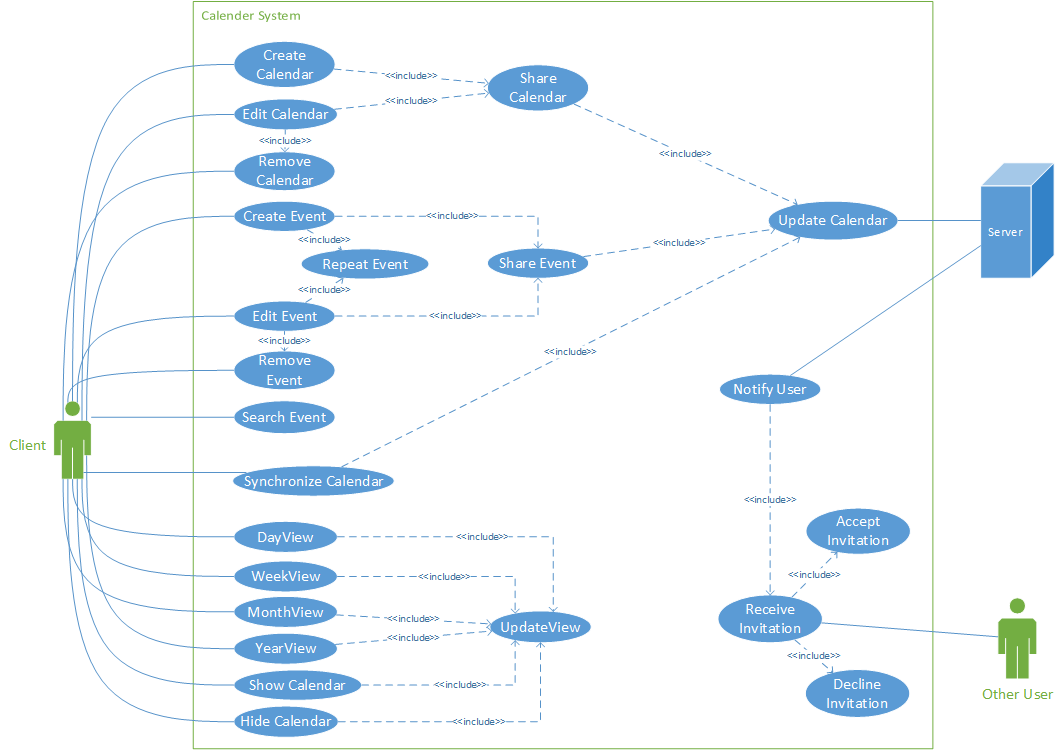
\includegraphics[width=110mm]{usecase.png}
\caption{UML Use Case Diagram \label{overflow}}
\end{figure}


\pagebreak \subsubsection{Use Case textual description}
This is the textual description for the "buy" use cases. 

\begin{usecase}

\addtitle{Use case name}{BuyOneWayTicket, \newline BuyWeeklyCard, \newline BuyMonthlyCard} 

\addfield{Participating Actors:}{Initiated by Traveler \newline Communicates with Central Computer}

\addscenario{Flow of events:}{
	\item The Traveler chooses to buy a ticket
	\item Tickettypes are presented
	\item The Traveler selects one of the three tickettypes
	\item Total amount is displayed
	\item The Traveler inserts money
	\item The amount inserted is checked. If the correct amount is inserted then the Central Computer prints out the ticket
	\item Central Computer resets when the purchase is completed
}

\additemizedfield{Entry conditions:}{
	\item The Traveler chooses to buy a ticket on the Ticket Machine
}

\additemizedfield{Exit conditions:}{
	\item The ticket is printed out OR
	\item Transaction is aborted OR
	\item The Ticket Machine times out. 
}

\additemizedfield{Quality requirements:}{
	\item The Ticket Machine can print tickets out
	\item Notify if the machine is out of paper
	\item Notify if the machine is out of money
}

\caption{Textual Description \label{overflow}}
\end{usecase}



\pagebreak \section*{Class Diagram}

A Class Diagram describes the structure of the system. 

The UserInput class is linked to Ticket class. The Ticket class is inherited by three classes which represent the three tickettypes. These tickettypes are linked to Transaction class. The UserInput class is also linked to the CentralComputer.

\begin{figure}[ht!]
\centering
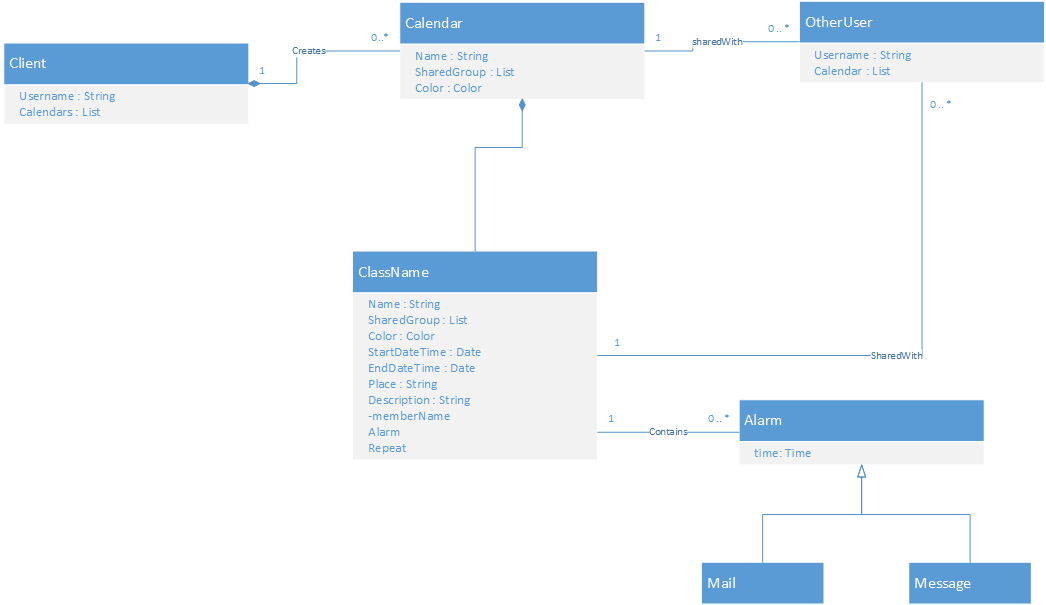
\includegraphics[width=160mm]{class.png}
\caption{UML Class Diagram \label{overflow}}
\end{figure}

\pagebreak \section*{Sequence Diagram}

This Sequence diagram illustrates time vertically and horizontally how the objects participate in the interaction when a ticket is bought.

*Some methods are not included in the Class Diagram. The Display class is also not included in the class Diagram.

\begin{itemize}
	\item pressBuyTicket() should invoke method chooseTicket() in the display
	\item then the tickettype is selected with pressTicketType()
	\item amount() shows the price of the selected tickettype in display.
	\item when money is inserted the amount is checked. 
	\item the Central Computer invokes PurchaseComplete() method if the correct amount is inserted and then resets.
\end{itemize}

\begin{figure}[ht!]
\centering
\includegraphics[width=160mm]{sequence.png}
\caption{UML Sequence Diagram \label{overflow}}
\end{figure}


\pagebreak \section*{Activity Diagram}

The action Ticket Purchase is followed by a decision which represents the set of possible outcomes. Each tickettype corresponds to a possible outcome. Amount is the activity where the ticket is paid for, which results in the last action Complete.

\begin{figure}[ht!]
\centering
\includegraphics[width=160mm]{activity.png}
\caption{UML Activity Diagram \label{overflow}}
\end{figure}


\end{document}